\documentclass[a4paper]{article}

%%%%%%%%%%%%%%%%%%%%%%%%%%%%%%%%%%%%%%%%%%%%%%%%%%%%%%%%%%%%%%%%%%%%%%%%%%%%%%%%%%%%%%%%%%%%%%%%%%%%
% Environment Setting
%%%%%%%%%%%%%%%%%%%%%%%%%%%%%%%%%%%%%%%%%%%%%%%%%%%%%%%%%%%%%%%%%%%%%%%%%%%%%%%%%%%%%%%%%%%%%%%%%%%%
\usepackage{fullpage}
\usepackage{graphicx}
\usepackage{color}
\usepackage{fancyhdr}
\usepackage{url}
\usepackage{amsmath,bm}
\usepackage{amssymb}
\usepackage{amsthm}
\usepackage{amsfonts}
\usepackage[round]{natbib}
\usepackage{enumitem,xcolor}
\usepackage[multiple]{footmisc}

\usepackage[
 pdftitle={Capstone Proposal - Udacity Machine Learning Nanodegree},
 pdfsubject={Machine Learning, Reinforcement Learning, Deep Learning, Artificial Intelligence, Games},
 pdfauthor={Peng Xu},
 pdfpagemode=UseOutlines,
 pdfborder= {0 0 1.0},
 bookmarks,
 bookmarksopen,
 colorlinks=true,
 citecolor=blue,
 linkcolor=blue, %
 linkbordercolor=blue, %
 urlcolor=blue, %
]{hyperref}

\usepackage[labelfont=bf]{caption}

\usepackage[utf8]{inputenc}

% Default fixed font does not support bold face
\DeclareFixedFont{\ttb}{T1}{txtt}{bx}{n}{8} % for bold
\DeclareFixedFont{\ttm}{T1}{txtt}{m}{n}{8}  % for normal

%%%%%%%%%%%%%
% EQUATIONS %
%%%%%%%%%%%%%

% ArgMin
\DeclareMathOperator*{\argmin}{\arg\!\min}

% ArgMax
\DeclareMathOperator*{\argmax}{\arg\!\max}

% Custom colors
\usepackage{color}
\definecolor{deepblue}{rgb}{0,0,0.5}
\definecolor{deepred}{rgb}{0.6,0,0}
\definecolor{deepgreen}{rgb}{0,0.5,0}
\definecolor{coolblue}{HTML}{101094}

\usepackage{listings}

\definecolor{codebg}{RGB}{238,238,238}

% Python style for highlighting
\newcommand\pythonstyle{\lstset{
    language=Python,
    basicstyle=\ttm,
    otherkeywords={},             % Add keywords here
    keywordstyle=\ttm\color{coolblue},
    emph={MyClass},          % Custom highlighting
    emphstyle=\ttm\color{deepred},    % Custom highlighting style
    stringstyle=\color{deepgreen},
    frame=tb,                         % Any extra options here
    framesep=10pt,
    framexleftmargin=10pt,
    backgroundcolor=\color{codebg},
    rulecolor=\color{codebg},
    aboveskip=15pt,
    belowskip=15pt,
    showstringspaces=false            % 
}}


% Python environment
\lstnewenvironment{python}[1][] {
    \pythonstyle
    \lstset{#1}
}{}

% \setmonofont[Color={0019D4}]{Courier New}


% Python for external files
\newcommand\pythonexternal[2][]{{
\pythonstyle
\lstinputlisting[#1]{#2}}}

% Python for inline
\newcommand\pythoninline[1]{{\pythonstyle\lstinline!#1!}}

\graphicspath{ {../images/} }
%%%%%%%%%%%%%%%%%%%%%%%%%%%%%%%%%%%%%%%%%%%%%%%%%%%%%%%%%%%%%%%%%%%%%%%%%%%%%%%%%%%%%%%%%%%%%%%%%%%%


%%%%%%%%%%%%%%%%%%%%%%%%%%%%%%%%%%%%%%%%%%%%%%%%%%%%%%%%%%%%%%%%%%%%%%%%%%%%%%%%%%%%%%%%%%%%%%%%%%%%
% Main Text begins here
%%%%%%%%%%%%%%%%%%%%%%%%%%%%%%%%%%%%%%%%%%%%%%%%%%%%%%%%%%%%%%%%%%%%%%%%%%%%%%%%%%%%%%%%%%%%%%%%%%%%
\begin{document}
%%%%%%%%%%%%%%%%%%%%%%%%%%%%%%%%%%%%%%%%%%%%%%%%%%%%%%%%%%%%%%%%%%%%%%%%%%%%%%%%%%%%%%%%%%%%%%%%%%%%


%%%%%%%%%%%%%%%%%%%%%%%%%%%%%%%%%%%%%%%%%%%%%%%%%%%%%%%%%%%%%%%%%%%%%%%%%%%%%%%%%%%%%%%%%%%%%%%%%%%%
% Tile Block
%%%%%%%%%%%%%%%%%%%%%%%%%%%%%%%%%%%%%%%%%%%%%%%%%%%%%%%%%%%%%%%%%%%%%%%%%%%%%%%%%%%%%%%%%%%%%%%%%%%%
\title{Machine Learning Nanodegree \\ Capstone Project \\ A Game Bot trained with Deep Q-Learning }
\author{Peng Xu}
\date{February 14, 2016}
\maketitle
%%%%%%%%%%%%%%%%%%%%%%%%%%%%%%%%%%%%%%%%%%%%%%%%%%%%%%%%%%%%%%%%%%%%%%%%%%%%%%%%%%%%%%%%%%%%%%%%%%%%


%%%%%%%%%%%%%%%%%%%%%%%%%%%%%%%%%%%%%%%%%%%%%%%%%%%%%%%%%%%%%%%%%%%%%%%%%%%%%%%%%%%%%%%%%%%%%%%%%%%%
% I. Definition (approx. 1-2 pages)
%%%%%%%%%%%%%%%%%%%%%%%%%%%%%%%%%%%%%%%%%%%%%%%%%%%%%%%%%%%%%%%%%%%%%%%%%%%%%%%%%%%%%%%%%%%%%%%%%%%%
\section{Definition}

%%%%%%%%%%%%%%%%%%%%%%%%%%%%%%%%%%%%%%%%%%%
\subsection{Project Overview}

% Reinforcement Learning
Reinforcement Learning is a type of machine learning that allows you to create AI agents that learn from the environment by interacting with it. Just like how we learn to ride a bicycle, this kind of AI learns by trial and error. As seen in Figure 1, the brain_matrix_library represents the AI agent, which acts on the environment. After each action, the agent receives the feedback. The feedback consists of the reward and next state of the environment. The reward is usually defined by a human. If we use the analogy of the bicycle, we can define reward as the distance from the original starting point.

\begin{figure}[h]
\centering
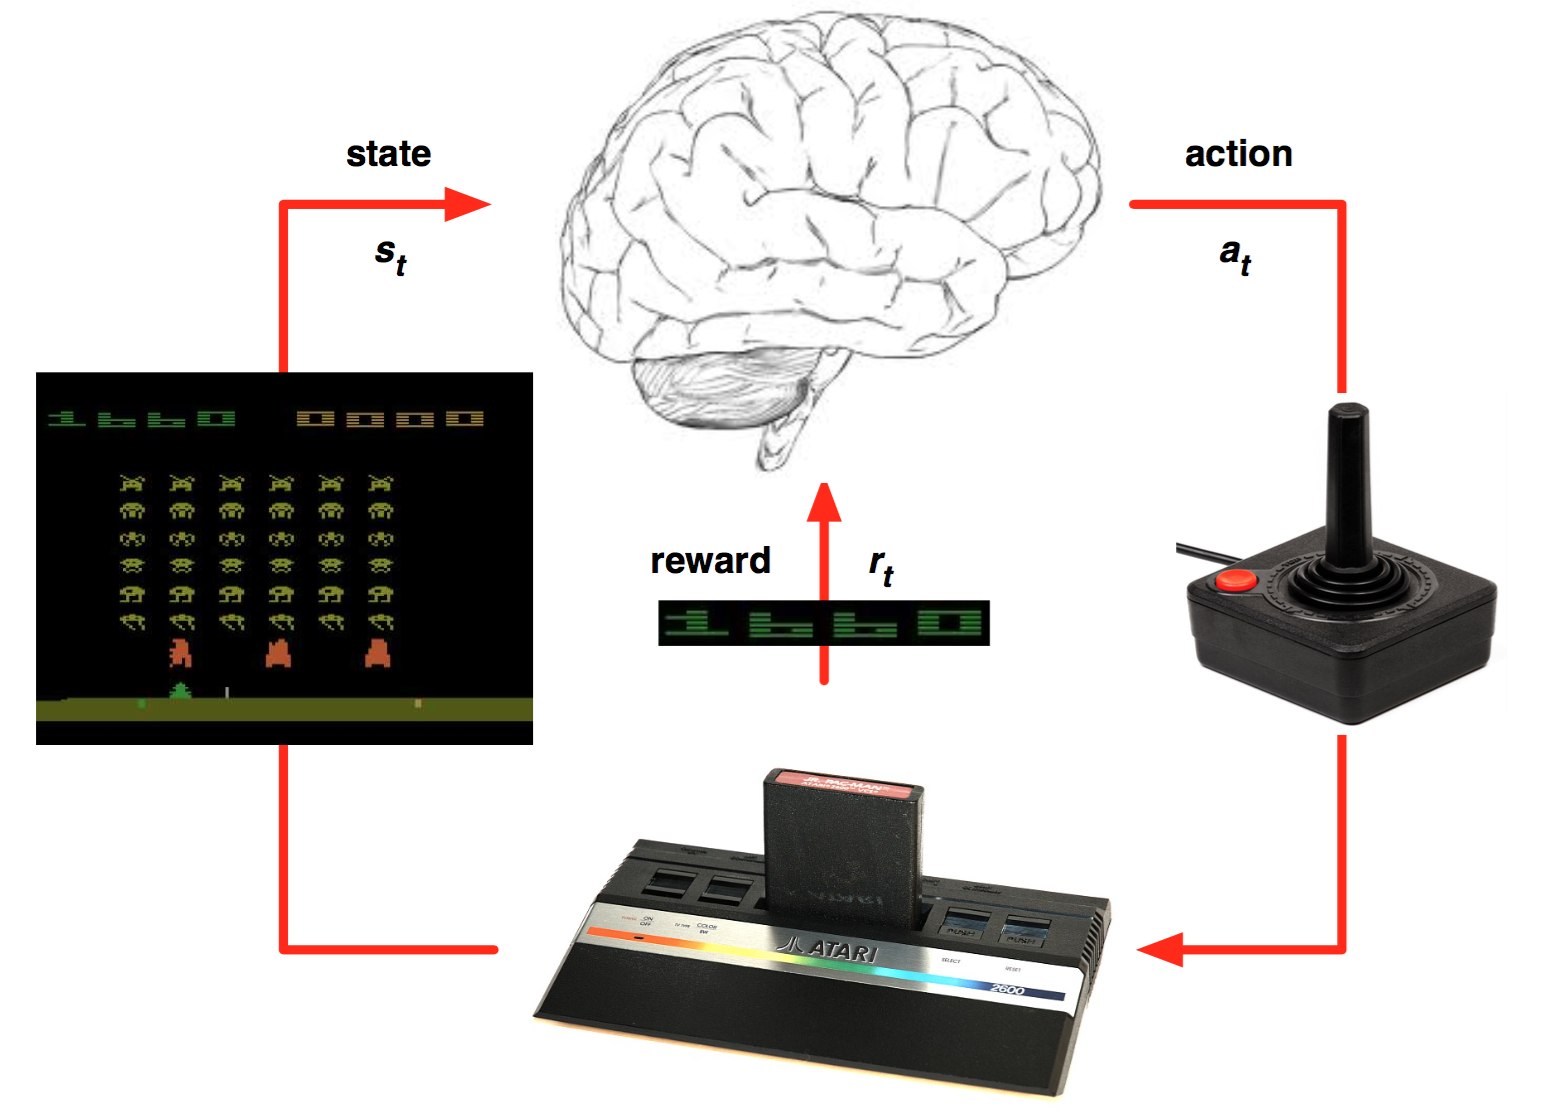
\includegraphics[width=0.5\textwidth]{rl}
\caption{How an agent interacts with the environment.}
\end{figure}

% Deep Reinforcement Learning
Google's DeepMind published its famous paper Playing Atari with Deep Reinforcement Learning, in which they introduced a new algorithm called Deep Q Network (DQN for short) in 2013. It demonstrated how an AI agent can learn to play games by just observing the screen without any prior information about those games. The result turned out to be pretty impressive. This paper opened the era of what is called ?deep reinforcement learning?, a mix of deep learning and reinforcement learning.

%%%%%%%%%%%%%%%%%%%%%%%%%%%%%%%%%%%%%%%%%%%
\subsection{Problem Statement}
\label{subsec:problem-statement}

In this project, a deep reinforcement learning method, Deep Q Network, would be implemented and applied to play a Coast Racer game in OpenGym / Universe using TensorFlow.

% Q Learning
Q-learning, a model-free online off-policy algorithm, whose main strength is that it is able to compare the expected utility of the available actions without requiring a model of the environment. In Q-Learning Algorithm, there is a function called Q Function, which is used to approximate the reward based on a state. We call it Q(s,a), where Q is a function which calculates the expected future value from state s and action a. Similarly in Deep Q Network algorithm, we use a neural network to approximate the reward based on the state. We will discuss how this works in detail.

% OpenAI Gym and Universe
OpenAI Gym is a toolkit for reinforcement learning research. It includes a growing collection of benchmark problems that expose a common interface, and a website where people can share their results and compare the performance of algorithms. Universe is a software platform for measuring and training an AI's general intelligence across the world's supply of games, websites and other applications. Universe allows an AI agent to use a computer like a human does: by looking at screen pixels and operating a virtual keyboard and mouse. We must train AI systems on the full range of tasks we expect them to solve, and Universe lets us train a single agent on any task a human can complete with a computer. With Universe, any program can be turned into a Gym environment. Universe works by automatically launching the program behind a VNC remote desktop. Hundreds of games have been translated into Gym environments and are ready for reinforcement learning, which mostly can be freely run with the universe Python library as follows:

\begin{python}
import gym
import universe # register Universe environments into Gym

env = gym.make('flashgames.DuskDrive-v0') # any Universe environment ID here
observation_n = env.reset()

while True:
  # agent which presses the Up arrow 60 times per second
  action_n = [[('KeyEvent', 'ArrowUp', True)] for _ in observation_n]
  observation_n, reward_n, done_n, info = env.step(action_n)
  env.render()
\end{python}

% Coast Racer Game
Among the several racing car games provided in Universe, the Coaster Racer flash game arose in front of me since it could be a typical simulation of Autonomous Driving, in which a vehicle is simply controlled by 3 inputs, left, right, forward. It is expected that the racing car can learn a smart driving behavior after a series of training steps leading to a maximal reward or namely score here. The trained bot for the Coaster Racer flash game will determines whether it should turn and which way it turns.

% Q function
\textbf{Target function:}

$Q^\pi : \mathcal{S} \times \mathcal{A} \to \mathbb{R}$, where $\mathcal{S}$ is the set of \emph{states} and $\mathcal{A}$ is the set of \emph{actions} (turn left, forward or turn right), and $\mathbb{R}$ represents the value of being in a state $s \in \mathcal{S}$, applying a action $a \in \mathcal{A}$, and following policy $\pi$ thereafter.

\textbf{Target function representation:}

Deep neural network.

Therefore, I seek to build a Q-learning agent trained via a deep convolutional neural network to approximate the optimal action-value function:

\begin{equation}
Q^*(s,a) = \max\limits_\pi Q^\pi(s,a), \forall s \in \mathcal{S}, a \in \mathcal{A}
\end{equation}

\noindent which is the maximum sum of rewards achievable by a behavior policy $\pi$.

%%%%%%%%%%%%%%%%%%%%%%%%%%%%%%%%%%%%%%%%%%%
\subsection{Metrics}

This metric consists in playing a high number of games (e.g. 100,000) against another agent (e.g. a random agent), and calculating the average of games won by the agent that uses the learned value function.
        
%%%%%%%%%%%%%%%%%%%%%%%%%%%%%%%%%%%%%%%%%%%%%%%%%%%%%%%%%%%%%%%%%%%%%%%%%%%%%%%%%%%%%%%%%%%%%%%%%%%%


%%%%%%%%%%%%%%%%%%%%%%%%%%%%%%%%%%%%%%%%%%%%%%%%%%%%%%%%%%%%%%%%%%%%%%%%%%%%%%%%%%%%%%%%%%%%%%%%%%%%
% II. Analysis (approx. 2-4 pages)
%%%%%%%%%%%%%%%%%%%%%%%%%%%%%%%%%%%%%%%%%%%%%%%%%%%%%%%%%%%%%%%%%%%%%%%%%%%%%%%%%%%%%%%%%%%%%%%%%%%%
\section{Analysis}

%%%%%%%%%%%%%%%%%%%%%%%%%%%%%%%%%%%%%%%%%%%
\subsection{Data Exploration}

By using a Deep Q-Learning model, there is no need to use an external dataset since the data are captured along with training. 

%%%%%%%%%%%%%%%%%%%%%%%%%%%%%%%%%%%%%%%%%%%
\subsection{Exploratory Visualization}
Skip.

%%%%%%%%%%%%%%%%%%%%%%%%%%%%%%%%%%%%%%%%%%%
\subsection{Coaster Racer Environment}

%%%%%%%%%%%%%%%%%%%%%%%%%%%%%%%%%%%%%%%%%%%
\subsection{Algorithms and Techniques}

To tackle the problem described in \hyperref[subsec:problem-statement]{Section \ref*{subsec:problem-statement}}, we will use Reinforcement learning with Deep Learning to automatically learn evaluation functions by playing games by itself. Unlike other approaches that need a very large dataset, this approach will try to learn to play games without any domain knowledge (no dataset will be used). This is a promising approach for creating game-playing algorithms for playing other two-player games of perfect information.

%%%%%%%%%%%%%%%%%%%%%%%%%%%%%%%%%%%%%%%
\subsubsection{Markov Decision Process}
%%%%%%%%%%%%%%%%%%%%%%%%%%%%%%%%%%%%%%%

A \emph{Markov decision process} (MDP) consist of four elements:

\begin{itemize}

    \item $\mathcal{S}$ is the set of \emph{states} (state space).

    \item $\mathcal{A}$ is the set of \emph{actions} (action space). The set of actions that are
        available in some particular state $s_t \in \mathcal{S}$ is denoted $\mathcal{A}(s_t)$.

    \item $ T : \mathcal{S} \times \mathcal{A} \times \mathcal{S} \to \mathbb{R}$ is the
      \emph{transition function}, which is the probability given we are in state $s_t \in
      \mathcal{S}$, take action $a_t \in \mathcal{A}(s_t)$ and we will transition to state $s_{t+1}
      \in \mathcal{S}$.

    \item $ R : \mathcal{S} \times \mathcal{A} \times \mathcal{S} \to \mathbb{R}$ is the
      \emph{reward function}, which is the immediate reward received when in state $s_t \in
      \mathcal{S}$ action $a_t \in \mathcal{A}$ is taken and the MDP transitions to state $s_{t+1}
      \in \mathcal{S}$. However, it is also possible to define it either as $ R : \mathcal{S} \times
      \mathcal{A} \to \mathbb{R}$ or $R : \mathcal{S} \to \mathbb{R}$. The first one gives rewards
      for performing an action $a_t$ in a particular state $s_t$, and the second gives rewards when
      transitioning to state $s_{t+1}$.

\end{itemize}

%%%%%%%%%%%%%%%%%%%%%%%%%%%
\subsubsection{Environment}
%%%%%%%%%%%%%%%%%%%%%%%%%%%

In the reinforcement learning problem an agent does not have access to the dynamics (reward and
transition functions) of the MDP. However, it interacts with an \emph{environment}
 by way of three signals: a \emph{state}, which describes the
state of the environment, an \emph{action}, which allows the agent to have some impact on the
environment, and a \emph{reward}, which provides the agent with feedback on its immediate
performance.

%%%%%%%%%%%%%%%%%%%%%%
\subsubsection{Policy}
%%%%%%%%%%%%%%%%%%%%%%

In an MDP, the agent acts according to a policy $\pi$ , which maps
each state $s \in \mathcal{S}$ to an action $a \in \mathcal{A}(s)$. A policy that specifies a unique
action to be performed is called a \emph{deterministic} policy, and is defined as $\pi : \mathcal{S}
\rightarrow \mathcal{A}$.

The interaction between the policy used by the agent and the environment works as follows. First, it
starts at an \emph{initial state} $s_0$. Then, the policy $\pi$ selects an action $a_0 = \pi(s_0)$
from the set of available actions $\mathcal{A}(s_0)$, and the action is executed. The environment
transitions to a new state $s_1$ based on the transition function $T$ with probability
$T(s_0,a_0,s_1)$, and a reward $r_0 = R(s_0, a_0, s_1)$ is received. This process continues,
producing a \emph{trajectory} of experience $s_0, a_0, s_1, r_1, a_1, s_2, r_2, a_2, \dots$, and the
process ends in a \emph{terminal state} $s_T$ and is restarted in the initial state.

We use three types of policies in this project:

\begin{itemize}

    \item \textbf{Random.} Selects actions uniformly at random
       .

    \item \textbf{Greedy.} Selects the \emph{max action}, which is the greedy
                           action with the highest value,

        \begin{equation}
            \pi_{\textrm{greedy}}(s) = \argmax_{a \in \mathcal{A}(s)} Q(s, a)
        \end{equation}

    \item \textbf{$\epsilon$-greedy.} Selects the best action for a proportion
        $1 - \epsilon$ of the trials, and another action is randomly selected (with
        uniform probability) for a proportion,

        \begin{equation}
            \pi_{\epsilon}(s) = \left\{
             \begin{array}{lr}
                 \pi_{\textrm{rand}}(s,a) & \text{if } rand() < \epsilon\\
                 \pi_{\textrm{greedy}}(s,a) & \text{otherwise}
             \end{array}
           \right.
        \end{equation}

        where $\epsilon \in [0, 1]$ and $rand()$ returns a random number from a
        uniform distribution $\in [0, 1]$.

\end{itemize}

%%%%%%%%%%%%%%%%%%%%%%%%%%%%%%%
\subsubsection{Value Functions}
%%%%%%%%%%%%%%%%%%%%%%%%%%%%%%%

Most of the algorithms for solving MDPs (computing optimal policies) do it by learning a \emph{value
function}. A value function estimates what is good for an
agent over the long run. It estimates the expected outcome from any given state, by summarizing the
total amount of reward that an agent can expect to accumulate into a single number. Value functions
are defined for particular policies.

The \emph{state value function} (or V-function), is the expected return when starting in state $s$
and following policy $\pi$ thereafter~\citep{Sutton1998RL},
%
\begin{equation}
V^\pi(s) = \mathbb{E}_\pi \left[R_t | s_t = s \right]
\end{equation}

The \emph{action value function} (or Q-function), is the expected return after selecting action $a$
in state $s$ and then following policy $\pi$,
%
\begin{equation}
Q^\pi(s,a) = \mathbb{E}_\pi \left[ R_t | s_t = s, a_t = a \right]
\end{equation}

The \emph{optimal value function} is the unique value function that maximises the value of every
state, or state-action pair,
%
\begin{eqnarray}
Q^*(s,a) & = & \max\limits_\pi Q^\pi(s,a), \forall s \in \mathcal{S}, a \in \mathcal{A}
\end{eqnarray}

An \emph{optimal policy} $\pi^*(s,a)$ is a policy that maximises the action value function from
every state in the MDP,
%
\begin{equation}
    \pi^*(s,a) = \argmax_\pi Q^\pi(s, a)
\end{equation}

%%%%%%%%%%%%%%%%%%%%%%%%%%
\subsubsection{Q-learning}
%%%%%%%%%%%%%%%%%%%%%%%%%%

One of the most basic and popular methods to estimate action-value functions is the
\emph{Q-learning} algorithm~ .
It is model-free online off-policy algorithm, whose main strength is that it is able to compare the
expected utility of the available actions without requiring a model of the environment. Q-learning
works by learning an action-value function that gives the expected utility of taking a given action
in a given state and following a fixed policy thereafter. The update rule uses action-values and a
built-in max-operator over the action-values of the next state in order to update $Q(s_t, a_t)$ as
follows,

\begin{equation}
Q(s_t,a_t) \gets Q(s_t,a_t) + \alpha \left[r_{t+1} + \gamma \max_a Q(s_{t+1},a) - Q(s_t,a_t)\right]
\end{equation}

The agent makes a step in the environment from state $s_t$ to $s_{t+1}$ using action $a_t$ while
receiving reward $r_t$. The update takes place on the action-value $a_t$ in the state $s_t$ from
which this action was executed. This version of Q-learning works well for tasks with a small a
state-space, since it uses arrays or tables with
one entry for each state-action pair.

%%%%%%%%%%%%%%%%%%%%%%%%%%%%%%%%%%%%%%
\subsubsection{Approximate Q-learning}
%%%%%%%%%%%%%%%%%%%%%%%%%%%%%%%%%%%%%%

In many cases in which there are far more states than could possibly be entries in a table we need
to use function approximation. Approximate Q-learning consists in parameterizing an approximate
action-value function, $Q(s,a;\theta_i) \approx Q(s,a)$, in which $\theta_i$ are the parameters
(weights) of the action-value function at iteration $i$. Usually the number of parameters of a
function approximator is much less than the state space, which means that a change in one parameter
can change many Q-values, as opposed to just one as in the tabular case.

%%%%%%%%%%%%%%%%%%%%%%%%%%%%%%%%%
\subsubsection{Experience Replay}
%%%%%%%%%%%%%%%%%%%%%%%%%%%%%%%%%

Reinforcement learning is known to be unstable or even to diverge when a nonlinear function
approximator such as a neural network is used to represent the action-value function. One trick to
make it work is to use \emph{experience replay}~, which consists in storing the experiences
$(s_t, a_t, r_t, s_{t+1})$ at each time step $t$ in a data set $D_t=\{e_1,\dots,e_t\}$. During the
training of approximate Q-learning random minibatches from the replay memory are used instead of the
most recent transition. This breaks the similarity of subsequent training samples, which otherwise
might drive the network into a local minimum. The \mbox{Q-learning} update at iteration $i$ uses the
following loss function~\citep{Mnih2015AtariNature}:

\begin{equation}
L_i(\theta_i) = \mathbb{E}_{(s, a, r, s') \sim U(D)} \\
                \left[\left(r + \gamma \max_{a'} Q(s',a', \theta^-_i) - Q(s,a;\theta)\right)^2\right]
\end{equation}
where $(s, a, r, s') \sim U(D)$ is a sample minibatch of experience drawn uniformly at random from
the memory pool of stores experiences.

%%%%%%%%%%%%%%%%%%%%%%%%%
\subsubsection{Self-play}
%%%%%%%%%%%%%%%%%%%%%%%%%

Self-play  is by far the most popular
training method for games. It is a single policy $\pi(s,a)$ that is used by both players in a
two-player game, $\pi_1(s,a) = \pi_2(s,a) = \pi(s,a)$. The first reason for its popularity is that
training is quickest if the learner's opponent is roughly equally strong, and that definitely holds
for self-play. As a second reason for popularity, there is no need to implement or access a
different agent with roughly equal playing strength. However, self-play has several drawbacks, with
the main one being that a single opponent does not provide sufficient
exploration~.

%%%%%%%%%%%%%%%%%%%%%%%%%%%%%%%%%%%%%%%%%%%%%
\subsubsection{Convolutional Neural Networks}
%%%%%%%%%%%%%%%%%%%%%%%%%%%%%%%%%%%%%%%%%%%%%

Convolutional Neural Networks~, or CNNs, are a special type of neural network that
has a known grid-like topology. Like most other neural networks they are trained with a variant of
the backpropagation algorithm. CNNs strengh is pattern recognition directly from pixels of images
with minimal processing. We use a convolutional network as a function approximator for the board of
Connect 4, since the board can be
thought of as a 2-D grid of pixels (discs in this case).

%%%%%%%%%%%%%%%%%%%%%%%%%%%%%%%%%%%%%%%%%%%
\subsection{Benchmark}

This benchmark consists in playing against an agent that takes uniformly random moves. This is the most basic benchmark, but first we have to be sure that our learned evaluation function can play better than a random agent before moving into a harder benchmark. Also, this will help us to detect bugs in the code and algorithms: if a learned value function does not play significantly better than a random agent, is not learning. The idea is to test against this benchmark using Alpha-beta pruning at 1, 2 and 4-ply search.

%%%%%%%%%%%%%%%%%%%%%%%%%%%%%%%%%%%%%%%%%%%%%%%%%%%%%%%%%%%%%%%%%%%%%%%%%%%%%%%%%%%%%%%%%%%%%%%%%%%%

%%%%%%%%%%%%%%%%%%%%%%%%%%%%%%%%%%%%%%%%%%%%%%%%%%%%%%%%%%%%%%%%%%%%%%%%%%%%%%%%%%%%%%%%%%%%%%%%%%%%
% III. Methodology (approx. 3-5 pages)
%%%%%%%%%%%%%%%%%%%%%%%%%%%%%%%%%%%%%%%%%%%%%%%%%%%%%%%%%%%%%%%%%%%%%%%%%%%%%%%%%%%%%%%%%%%%%%%%%%%%
\section{Methodology}

Q-learning, a model-free online off-policy algorithm, whose main strength is that it is able to compare the expected utility of the available actions without requiring a model of the environment:

\begin{equation}
        Q(s_t, a_t) \gets Q(s_t, a_t) + \alpha [r_{t+1} + \gamma \max_a Q(s_{t+1}, a) - Q(s_t, a_t)]
\end{equation}

%%%%%%%%%%%%%%%%%%%%%%%%%%%%%%%%%%%%%%%%%%%
\subsection{Data Preprocessing}

The original input is a 3 dimensional RGB image or matrix and the data preprocessing here is to downsize the matrix so the model can focus on the core features. The image is gray scaled and resized to as smaller size, [160, 120].

%%%%%%%%%%%%%%%%%%%%%%%%%%%%%%%%%%%%%%%%%%%
\subsection{Implementation}

Before getting started, we need to install Docker. Docker is a tool that lets you run virtual machines on the local computer. I created an image wrapping up everything necessary, like TensorFlow, OpenCV, Gym and Universe.

%%%%%%%%%%%%%%%%%%%%%%%%%%%%%%%%%%%%%%%%%%%
\subsection{Refinement}

%%%%%%%%%%%%%%%%%%%%%%%%%%%%%%%%%%%%%%%%%%%%%%%%%%%%%%%%%%%%%%%%%%%%%%%%%%%%%%%%%%%%%%%%%%%%%%%%%%%%


%%%%%%%%%%%%%%%%%%%%%%%%%%%%%%%%%%%%%%%%%%%%%%%%%%%%%%%%%%%%%%%%%%%%%%%%%%%%%%%%%%%%%%%%%%%%%%%%%%%%
% IV. Results (approx. 2-3 pages)
%%%%%%%%%%%%%%%%%%%%%%%%%%%%%%%%%%%%%%%%%%%%%%%%%%%%%%%%%%%%%%%%%%%%%%%%%%%%%%%%%%%%%%%%%%%%%%%%%%%%
\section{Results}

%%%%%%%%%%%%%%%%%%%%%%%%%%%%%%%%%%%%%%%%%%%
\subsection{Model Evaluation and Validation}

%%%%%%%%%%%%%%%%%%%%%%%%%%%%%%%%%%%%%%%%%%%
\subsection{Justification}

%%%%%%%%%%%%%%%%%%%%%%%%%%%%%%%%%%%%%%%%%%%%%%%%%%%%%%%%%%%%%%%%%%%%%%%%%%
\subsubsection{Play withQ-learning}
%%%%%%%%%%%%%%%%%%%%%%%%%%%%%%%%%%%%%%%%%%%%%%%%%%%%%%%%%%%%%%%%%%%%%%%%%%



%%%%%%%%%%%%%%%%%%%%%%%%%%%%%%%%%%%%%%%%%%%%%%%%%%%%%%%%%%%%%%%%%%%%%%%%%%
\subsubsection{Learning to Play Connect 4 using Q-learning with a Deep Neural Network}
%%%%%%%%%%%%%%%%%%%%%%%%%%%%%%%%%%%%%%%%%%%%%%%%%%%%%%%%%%%%%%%%%%%%%%%%%%

Once we validated that our implementation of Q-learning is working and showed that it can learn a
tabular value function to play Tic-Tac-Toe we moved into the more complex Connect 4. In this game,
storing the Q-values for every board position in a lookup table is not feasible because of its huge
state space. Instead of using tabular Q-learning, we used approximate
Q-learning~ with a deep neural network
(DNN). This approach consists in
parameterizing an approximate action-value function, $Q(s,a;\theta_i) \approx Q(s,a)$, in which
$\theta_i$ are the weights of the neural network.

In some games it can be more efficient to consider the \emph{afterstate value} $V(s \circ a)$, which
is the state reached after taking action $a$ in state $s$, instead of the Q-value $Q(s,
a)$~\citep{Sutton1998RL}. We used this approach by using a DNN that takes the state of the board in
the input layer, as shown in \hyperref[fig:c4-dnn-input] {Figure~\ref*{fig:c4-dnn-input}}, and
outputs the value of being in that state, $V(s)$. After the input layer, we used convolutions with 4
layers of 64 filters of size $3\times3$ and rectified linear non-linearities. In addition to the
convolutions, we added a densely-connected layer with 256 units. Finally, the output layer has only
one unit that fires the value of the given board with a $tanh$ activation function to keep it in the
range $[-1, +1]$.

In this experiment our goal was to learn to play Connect 4
starting from 8-ply positions from the UCI Connect 4 dataset (\hyperref[sec:uci-c4]
{Section~\ref*{sec:uci-c4}}). In these positions we already know the game-theoretical outcome of the
game assuming perfect play from both players, however, we did not use the outcome for training (no
supervised learning), only for evaluation. This helped us to start every episode of Q-learning
training from different board positions, which is helpful to learn to generalize by seeing all kinds
of board positions.

In \hyperref[fig:c4-ql-dn-uci] {Figure~\ref*{fig:c4-ql-dn-uci}} we can see how the quality of the
target policy improved during training. The policy was evaluated during training every 500 episodes
by playing 3,000 games against a random player starting from randomly selected 8-ply positions from
the UCI Connect 4 dataset. The first 1,000 games started from positions where the outcome is a win
for the first player assuming perfect play from both sides. \hyperref[fig:c4-ql-dn-uci-wins]
{Figure~\ref*{fig:c4-ql-dn-uci-wins}} shows how the policy improved from a 56\% to a 94\% win rate
after 15,000 episodes. This makes sense because the matches started from favorable positions with
higher probability of winning for the first player. The next 1,000 games started from
game-theoretical draw positions (\hyperref[fig:c4-ql-dn-uci-draws]
{Figure~\ref*{fig:c4-ql-dn-uci-draws}}).  As expected, the win rate at the beginning was 50\%, but
then it went up to 92\%. Good improvement, but a little lower win rate than when starting from
favorable positions. Finally, the last 1,000 games (\hyperref[fig:c4-ql-dn-uci-losses]
{Figure~\ref*{fig:c4-ql-dn-uci-losses}}) started from unfavorable positions that are guaranteed wins
for the second player under optimal play from both sides. In this case the win rate before the
policy begins learning is 45\%, but then it went up to a 90\% win rate. This was also expected,
since we started at a disadvantage.

%%%%%%%%%%%%%%%%%%%%%%%%%%%%%%%%%%%%%%%%%%%%%%%%%%%%%%%%%%%%%%%%%%%%%%%%%%%%%%%%%%%%%%%%%%%%%%%%%%%%


%%%%%%%%%%%%%%%%%%%%%%%%%%%%%%%%%%%%%%%%%%%%%%%%%%%%%%%%%%%%%%%%%%%%%%%%%%%%%%%%%%%%%%%%%%%%%%%%%%%%
% V. Conclusion (approx. 1-2 pages)
%%%%%%%%%%%%%%%%%%%%%%%%%%%%%%%%%%%%%%%%%%%%%%%%%%%%%%%%%%%%%%%%%%%%%%%%%%%%%%%%%%%%%%%%%%%%%%%%%%%%
\section{Conclusion}

%%%%%%%%%%%%%%%%%%%%%%%%%%%%%%%%%%%%%%%%%%%
\subsection{Free-Form Visualization}

%%%%%%%%%%%%%%%%%%%%%%%%%%%%%%%%%%%%%%%%%%%
\subsection{Reflection}
The most difficult aspect of this project was that is extremely hard to stabilize reinforcement
learning with non-linear function approximators via self-play. There are plenty of tricks that can
be used and hyperparameters that need to be tuned to get it to work, such as:

\begin{itemize}

    \item \textbf{Q-learning}: exploration policy (random?, $\epsilon$-greedy?), discount factor,
        learning rate, number of episodes.

    \item \textbf{Experience Replay}: batch size, experience pool size.

    \item \textbf{Deep Neural Network}: mlp? convnets? number of layers, number of filters, number
        of kernels, optimizer (vanilla sgd, adam, rprop), learning rate, pooling, activation
        functions, etc.

    \item \textbf{$\epsilon$-greedy}: fixed $\epsilon$? decrease $\epsilon$? initial value for
        $\epsilon$?, how many episodes to decrease it? final value?

\end{itemize}

All these techniques and parameters were selected by trial and error, and no systematic grid search
was done due to the high computational cost. More than once it seemed that the implementation of the
algorithms and techniques was incorrect, and it turned out that the wrong parameters were being
used. A ``simple'' change such as decreasing $\epsilon$, or changing the neural network optimizer
made big changes in the performance of the value function.

%%%%%%%%%%%%%%%%%%%%%%%%%%%%%%%%%%%%%%%%%%%
\subsection{Improvement}
There are at least two aspects we can improve in the next stage,

\begin{enumerate}

    \item \textbf{Better benchmarks:} In most of this project we used simple benchmarkers, such as
        playing against random players. While testing against random is probably the first thing to
        test against (if you can't beat a random player your learning algorithm is not working), it
        would be better to find a few heuristics and better players that can be used for testing.

    \item \textbf{Incorporate other RL techniques:} The field of RL has been advancing fast in
        recent years. There are a few new and old techniques that I would like to try, such as
        asynchronous RL, double Q-learning, prioritized experience replay.

\end{enumerate}

%%%%%%%%%%%%%%%%%%%%%%%%%%%%%%%%%%%%%%%%%%%%%%%%%%%%%%%%%%%%%%%%%%%%%%%%%%%%%%%%%%%%%%%%%%%%%%%%%%%%


%%%%%%%%%%%%%%%%%%%%%%%%%%%%%%%%%%%%%%%%%%%%%%%%%%%%%%%%%%%%%%%%%%%%%%%%%%%%%%%%%%%%%%%%%%%%%%%%%%%%
% Reference (Bibliography)
%%%%%%%%%%%%%%%%%%%%%%%%%%%%%%%%%%%%%%%%%%%%%%%%%%%%%%%%%%%%%%%%%%%%%%%%%%%%%%%%%%%%%%%%%%%%%%%%%%%%
\bibliographystyle{unsrt}
\bibliography{bibliography}
%%%%%%%%%%%%%%%%%%%%%%%%%%%%%%%%%%%%%%%%%%%%%%%%%%%%%%%%%%%%%%%%%%%%%%%%%%%%%%%%%%%%%%%%%%%%%%%%%%%%


%%%%%%%%%%%%%%%%%%%%%%%%%%%%%%%%%%%%%%%%%%%%%%%%%%%%%%%%%%%%%%%%%%%%%%%%%%%%%%%%%%%%%%%%%%%%%%%%%%%%
% Document Ending
%%%%%%%%%%%%%%%%%%%%%%%%%%%%%%%%%%%%%%%%%%%%%%%%%%%%%%%%%%%%%%%%%%%%%%%%%%%%%%%%%%%%%%%%%%%%%%%%%%%%
\end{document}
%%%%%%%%%%%%%%%%%%%%%%%%%%%%%%%%%%%%%%%%%%%%%%%%%%%%%%%%%%%%%%%%%%%%%%%%%%%%%%%%%%%%%%%%%%%%%%%%%%%%

